% ============================================================================
% Lecture 13 (B12): OLG Models with DEQNs
% Deep Learning for Solving and Estimating Dynamic Models in Economics and Finance
% Course author: Simon Scheidegger
% ============================================================================

\documentclass[aspectratio=169,11pt]{beamer}

% ---------- Theme and colors ----------
\usecolortheme{dove}
\setbeamertemplate{navigation symbols}{}
\setbeamertemplate{footline}{%
  \hfill\usebeamerfont{page number in head/foot}%
  \usebeamercolor[fg]{normal text}%
  \insertframenumber\,/\,\inserttotalframenumber\kern1em\vskip4pt}
\setbeamerfont{frametitle}{size=\huge}

% ---------- Packages ----------
\usepackage[utf8]{inputenc}
\usepackage[T1]{fontenc}
\usepackage{lmodern}
\usepackage{amsmath,amssymb,amsfonts}
\usepackage{bm}
\usepackage{graphicx}
\usepackage{tikz}
\usetikzlibrary{shapes,arrows.meta,positioning,calc,fit,backgrounds,patterns,decorations.pathreplacing}
\usepackage{pgfplots}
\pgfplotsset{compat=1.18}
\usepackage{booktabs}
\usepackage{hyperref}
\usepackage{xcolor}

% ---------- Custom colors ----------
\definecolor{uzhblue}{rgb}{0,0,0.5}
\definecolor{uzhgreylight}{RGB}{236,238,241}
\definecolor{uzhgreydark}{RGB}{81,86,94}
\definecolor{harvardcrimson}{RGB}{153,0,0}
\definecolor{unil@blue}{RGB}{0,140,204}
\definecolor{unil@black}{RGB}{35,31,32}
\definecolor{darkgreen}{RGB}{0,100,0}
\definecolor{darkred}{RGB}{139,0,0}
\definecolor{softblue}{RGB}{70,130,180}
\definecolor{softorange}{RGB}{230,159,0}
\definecolor{softgreen}{RGB}{0,158,115}

% ---------- Set beamer colors ----------
\setbeamercolor{frametitle}{bg=uzhgreylight, fg=uzhblue}
\setbeamercolor{title}{fg=uzhblue}
\setbeamercolor{structure}{fg=uzhblue}
\setbeamercolor{block title}{bg=unil@blue, fg=white}
\setbeamercolor{block body}{bg=uzhgreylight}
\setbeamercolor{block title alerted}{bg=darkred,fg=white}
\setbeamercolor{block body alerted}{bg=red!5}
\setbeamercolor{block title example}{bg=darkgreen,fg=white}
\setbeamercolor{block body example}{bg=green!5}
\setbeamercolor{item}{fg=unil@black}
\setbeamercolor{normal text}{fg=unil@black}

% ---------- Emphasis and hyperlinks ----------
\newcommand{\emphc}[1]{\textcolor{harvardcrimson}{#1}}
\hypersetup{colorlinks,linkcolor=harvardcrimson,urlcolor=harvardcrimson}

% ---------- Math shortcuts ----------
\newcommand{\R}{\mathbb{R}}
\newcommand{\E}[1]{\mathbb{E}\!\left[#1\right]}
\newcommand{\N}{\mathcal{N}}
\newcommand{\Loss}{\mathcal{L}}
\newcommand{\st}{\text{s.t.}\ }
\newcommand{\ubr}[2]{\underbrace{#1}_{\text{\scriptsize #2}}}

% ---------- Title ----------
\title[Lecture 14 (B13)]{Lecture 14 (B13): Large OLG Benchmark --- 56 Cohorts (AGS 2022)}
\subtitle{Bond market, lifecycle capital, training diagnostics}
\author{Simon Scheidegger}
\institute{HEC, University of Lausanne}
\date{}
\begin{document}

% Custom command used in some "Finger Exercise" frame titles.
\providecommand{\exercisepause}{%
  \tikz[baseline=(X.base)]{\node[fill=darkgreen!80!black, text=white,
  rounded corners=2pt, inner sep=3pt, font=\scriptsize\bfseries](X){PAUSE};}}

{\setbeamercolor{background canvas}{bg=uzhgreylight}
\begin{frame}
\titlepage
\end{frame}
}

% --- About-this-lecture orientation ---
\begin{frame}{About this lecture}
\small
\begin{block}{What this lecture covers}
\begin{itemize}\itemsep2pt
  \item AGS 2022 benchmark: 56 cohorts, bond market, lifecycle capital
  \item DEQN architecture and equilibrium conditions for the larger model
  \item Training, consumption profiles by aggregate state, reading the diagnostics
\end{itemize}
\end{block}
\begin{block}{Builds on}
\begin{itemize}\itemsep2pt
  \item Lecture 13 (analytic 6-cohort OLG)
\end{itemize}
\end{block}
\begin{block}{Leads to}
\begin{itemize}\itemsep2pt
  \item Lecture 15 (heterogeneous agents and Young's method)
\end{itemize}
\end{block}
\end{frame}

\section{Part III: Benchmark 56-cohort OLG (AGS 2022 \S 3)}

% --- III.1 Setup -------------------------------------------------------
\begin{frame}{III.1 Setup --- the Leading Example of AGS (2022)}
\small
\begin{columns}[T]
\column{0.56\textwidth}
\emphc{Same recipe as Part II.  What changes:}
\begin{itemize}\itemsep1pt
    \item Agents live for $A = \emphc{56}$ periods (ages 25--80); one period = one year.
    \item CRRA utility $u(c) = c^{1-\gamma}/(1-\gamma)$ with $\gamma = 2$ (\emphc{not} log).
    \item \emphc{Hump-shaped labor endowment} $\ell^s$ (Kotlikoff-style; right panel).
    \item \emphc{Persistent} Markov shocks on $(\eta,\delta)$ (not i.i.d.).
    \item \emphc{Two assets}: capital $k^s$ and bonds $b^s$.
    \item \emphc{Two constraints}: borrowing $k'^s \ge 0$ and collateral $k'^s + \kappa b'^s \ge 0$.
    \item Capital adjustment costs $\Psi^s = \tfrac{\zeta}{2}(k'^s - r k^s)^2$.
\end{itemize}

\column{0.42\textwidth}
\centering
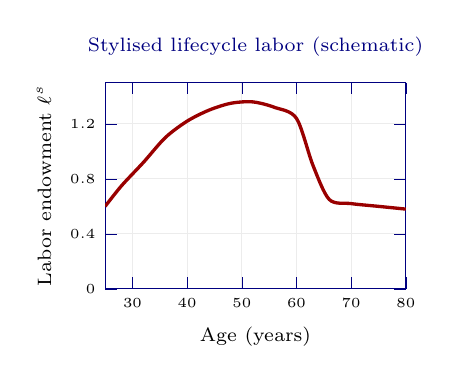
\begin{tikzpicture}
\begin{axis}[
    width=5.4cm, height=4.2cm,
    xlabel={Age (years)}, ylabel={Labor endowment $\ell^s$},
    xmin=25, xmax=80, ymin=0, ymax=1.5,
    xtick={30,40,50,60,70,80}, ytick={0, 0.4, 0.8, 1.2},
    grid=major, grid style={gray!15},
    axis line style={uzhblue}, tick style={uzhblue},
    label style={font=\scriptsize}, ticklabel style={font=\tiny},
    title style={font=\scriptsize, uzhblue},
    title={Stylised lifecycle labor (schematic)}
]
\addplot[harvardcrimson, very thick, smooth] coordinates {
    (25,0.60) (28,0.75) (32,0.92) (36,1.10) (40,1.22)
    (44,1.30) (48,1.35) (52,1.36) (56,1.32) (60,1.24)
    (63,0.90) (66,0.65) (70,0.62) (75,0.60) (80,0.58)
};
\end{axis}
\end{tikzpicture}

{\scriptsize \emphc{Schematic shape only}, rises through working years, drops sharply at retirement, low but nonzero after.  See AGS (2022) for the exact $\ell^s$ used in the notebook.}
\end{columns}
\end{frame}


% --- III.2 Households I ------------------------------------------------
\begin{frame}{III.2 Households --- Preferences and Savings Technology}
\small
An agent of age $s$ alive at $t$ maximises
\[
\E{\sum_{i=0}^{A-s} \beta^i \,u\!\bigl(c_{t+i}^{\,s+i}\bigr)}, \qquad u(c) = \frac{c^{1-\gamma}}{1-\gamma}, \qquad \gamma = 2. \qquad (1')
\]

\vspace{0.3em}
\textbf{Two saving instruments} (instead of one):
\begin{itemize}\itemsep2pt
    \item \emphc{Capital} $k_{t+1}^{\,s+1}$: yields gross return $r_{t+1}$ next period; incurs an \emphc{adjustment cost} $\Psi_t^s = \tfrac{\zeta}{2}(k_{t+1}^{\,s+1} - r_t k_t^{\,s})^2$.
    \item \emphc{Bonds} $b_{t+1}^{\,s+1}$: traded at price $q_t$ today, pay one unit of consumption next period. \emphc{Zero net supply}: $\sum_{s=1}^A b_t^s = 0$.
\end{itemize}

\vspace{0.3em}
Savings become next-period asset holdings ($\forall s \in \{1, \ldots, A-1\}$):
\[
k_{t+1}^{\,s+1} \;=\; a_{t,k}^{\,s}, \qquad b_{t+1}^{\,s+1} \;=\; a_{t,b}^{\,s}. \qquad (2')
\]
\end{frame}


% --- III.3 Households II -----------------------------------------------
\begin{frame}{III.3 Households --- Constraints, Budget, Boundary}
\small
\textbf{Two constraints on the capital--bonds pair $(k'^s, b'^s)$:}
\[
k'^s \;\ge\; 0 \quad (\text{borrowing constraint}), \qquad\quad
k'^s \;+\; \kappa\, b'^s \;\ge\; 0 \quad (\text{collateral constraint}).
\qquad (3')
\]

\vspace{0.4em}
\textbf{Budget constraint} of cohort $s$ (bonds enter at price $q_t$ on the left-hand side, pay off on the right):
\[
c_t^{\,s} \;+\; k_{t+1}^{\,s+1} \;+\; q_t\, b_{t+1}^{\,s+1} \;+\; \Psi_t^s
\;=\; r_t\, k_t^{\,s} \;+\; b_t^{\,s} \;+\; \ell_t^{\,s}\, w_t.
\qquad (4')
\]

\vspace{0.4em}
\textbf{Boundary conditions} (born and die without assets):
\[
k_t^{\,1} = 0,\ b_t^{\,1} = 0; \qquad k_{t+1}^{\,A+1} = 0,\ b_{t+1}^{\,A+1} = 0.
\]

\vspace{0.3em}
{\footnotesize Bond parameter $\kappa \ge 0$ governs how much bond-short position capital collateralises; $\kappa = 0$ is a \emphc{hard} short-sale constraint on bonds.}
\end{frame}


% --- III.4 Firms & Markets ---------------------------------------------
\begin{frame}{III.4 Firms and Markets --- Adding the Bond Market}
\small
\textbf{Representative firm.}  Same Cobb--Douglas as Part II:
\[
f(K, L, z) \;=\; \eta(z)\, K^{\alpha}\, L^{1-\alpha} \;+\; K\bigl(1-\delta(z)\bigr).
\]
Labor now aggregates over the hump-shaped profile: $L_t = \sum_{s=1}^{A} \ell^s$ (a constant).

\vspace{0.5em}
\textbf{Markets cleared in equilibrium.}
\begin{enumerate}\itemsep2pt
    \item Labor: $L_t = \sum_{s=1}^{A} \ell^s$.
    \item Capital: $K_t = \sum_{s=1}^{A} k_t^{\,s}$.
    \item \emphc{Bonds (new): $\displaystyle 0 \;=\; \sum_{s=1}^{A} b_t^{\,s}.$}\quad (Zero net supply.)
\end{enumerate}

\vspace{0.3em}
\textbf{Aggregate shocks.}  $z_t \in \{1,\ldots,4\}$ as before, but transition $\pi^z$ is \emphc{persistent} (not i.i.d.): $(\eta, \delta)$ have their own Markov chains, tensor-producted.
\end{frame}


% --- III.5 Equilibrium definition --------------------------------------
\begin{frame}{III.5 Competitive Equilibrium --- Definition}
\small
\begin{block}{Definition 1' (competitive equilibrium, benchmark)}
Given initial conditions $z_0,\, \{k_0^{\,s}, b_0^{\,s}\}_{s=1}^{A-1}$, a competitive equilibrium is
a collection of choices $\bigl\{(c_t^s,\,k_t^{\,s+1},\,b_t^{\,s+1})_{s=1}^{A-1}\bigr\}_{t=0}^\infty$,
firm demands $(K_t, L_t)_{t \ge 0}$, and prices $(r_t, w_t, q_t)_{t\ge 0}$, such that:
\begin{enumerate}\itemsep1pt
    \item Households maximize $(1')$ subject to $(2')$--$(4')$.
    \item Firm maximises profits, same closed-form FOCs as Part II.
    \item \emphc{All three markets clear} every period: capital, labor, \emphc{bonds}.
\end{enumerate}
\end{block}

\vspace{0.3em}
{\footnotesize Relative to Part II: one new price ($q_t$), one new market-clearing condition (bonds), one new asset class per cohort in the choice vector.  Everything else is the same.}
\end{frame}


% --- III.6 Equilibrium conditions -------------------------------------
\begin{frame}{III.6 Equilibrium Conditions (Benchmark)}
\small
\textbf{Firm FOCs.}  Same closed form as Part II.

\vspace{0.3em}
\textbf{Two Euler equations per cohort}, for $s = 1, \ldots, A-1$:
\[
\text{(capital)}\;\;
u'(c_t^s) \cdot \bigl(1 + \zeta\,(k'^s - r_t k_t^s)\bigr) \;=\; \beta\,\E{u'(c_{t+1}^{s+1})\,r_{t+1}} \;+\; \lambda_{\text{b}}^s \;+\; \lambda_{\text{c}}^s,
\]
\[
\text{(bonds)}\;\;
u'(c_t^s)\cdot q_t \;=\; \beta\,\E{u'(c_{t+1}^{s+1})} \;+\; \kappa\,\lambda_{\text{c}}^s.
\]

\vspace{0.3em}
\textbf{Two KKT triples per cohort.}
\[
\lambda_{\text{b}}^s \ge 0,\quad k'^s \ge 0,\quad \lambda_{\text{b}}^s\cdot k'^s = 0;
\qquad
\lambda_{\text{c}}^s \ge 0,\quad k'^s + \kappa b'^s \ge 0,\quad \lambda_{\text{c}}^s\cdot (k'^s + \kappa b'^s) = 0.
\]

\vspace{0.3em}
\textbf{Terminal cohort.}  Age $A$: consume everything.

\vspace{0.4em}
{\footnotesize So per state we have $4(A-1)$ per-agent residuals + 1 bond market-clearing residual = $\bm{4\,(A-1) + 1}$ equations.}
\end{frame}


% --- III.7 Cost function ----------------------------------------------
\begin{frame}{III.7 The DEQN Cost Function (Benchmark)}
\footnotesize
\begin{block}{Five loss components, one cost function}
\vspace{-2pt}
\[
\Loss_{D_{\text{train}}}(\rho) \;=\; \frac{1}{|D_{\text{train}}|}\,\frac{1}{4(A-1)+1}\!
\sum_{x_j \in D_{\text{train}}}\!\Biggl[\;\sum_{s=1}^{A-1} R^{\,s}(x_j)^2 \;+\; \bigl(e_{\text{MC},b}(x_j)\bigr)^2\;\Biggr],
\]

\vspace{4pt}
\hrule
\vspace{4pt}
\[
\text{where}\;\;\;R^{\,s}(x_j)^2 \;:=\; \bigl(e_{\text{REE},k}^{\,s}\bigr)^2 + \bigl(e_{\text{REE},b}^{\,s}\bigr)^2 + \bigl(e_{\text{KKT},b}^{\,s}\bigr)^2 + \bigl(e_{\text{KKT},c}^{\,s}\bigr)^2.
\]
\vspace{-4pt}
\end{block}

\vspace{-2pt}
\textbf{Component map.}
\begin{itemize}\itemsep0pt
    \item $e_{\text{REE},k}^{\,s},\;e_{\text{REE},b}^{\,s}$: relative residuals of the capital and bond Euler equations.
    \item $e_{\text{KKT},b}^{\,s} = \lambda_{\text{b}}^s \cdot k'^s$: borrowing KKT.
    \item $e_{\text{KKT},c}^{\,s} = \lambda_{\text{c}}^s \cdot (k'^s + \kappa b'^s)$: collateral KKT.
    \item $e_{\text{MC},b} = \sum_{s=1}^{A} b_t^{\,s}$: bond market clearing.
\end{itemize}

\vspace{0.2em}
{\scriptsize With $A = 56$ this is \emphc{$4 \times 55 + 1 = 221$} loss terms per training state.  The structure is the same as Part II: squared equilibrium residuals.}
\end{frame}


% --- III.8 FREE --------------------------------------------------------
\begin{frame}{III.8 Functional Rational Expectations Equilibrium}
\small
\begin{exampleblock}{FREE for the benchmark}
\vspace{-3pt}
\[
f:\;\{1,\ldots,4\}\times \R^{A}\times \R^{A} \;\longrightarrow\; \R^{\,4(A-1)+1}
\]
\[
f\!\left(\!\begin{bmatrix} z_t \\ \bm{k}_t \\ \bm{b}_t \end{bmatrix}\!\right)
\;=\;
\begin{bmatrix}
\hat{k}_t'^1,\ldots,\hat{k}_t'^{A-1} \\
\hat\lambda_{b,t}^1,\ldots,\hat\lambda_{b,t}^{A-1} \\
\hat q_{t}^{1},\ldots,\hat q_{t}^{A-1} \\
\hat \mu_{t}^{1},\ldots,\hat \mu_{t}^{A-1} \\
\hat p_t
\end{bmatrix}^{\!\top}
\]
{\footnotesize Output blocks: capital savings; borrowing multipliers; collateral $\hat q^h \equiv \hat k'^h + \kappa\,\hat b'^h$; collateral multipliers; equilibrium bond price (one scalar).}
\vspace{-3pt}\end{exampleblock}

\textbf{Such that} $G\bigl([z_t, \bm{k}_t, \bm{b}_t],\,f([z_t, \bm{k}_t, \bm{b}_t])\bigr) = \bm{0}$ where $G$ stacks the $4(A-1)+1$ equations of III.6.

\vspace{0.3em}
{\footnotesize With $A = 56$: minimal state dim $=113$; the notebook input is $236$ after engineered aggregates and transition probabilities.  Output dim $=4\times55+1=\bm{221}$.  Bond holdings are recovered as $\hat b'^h=(\hat q^h-\hat k'^h)/\kappa$, and softplus enforces $\hat k'^h,\hat\lambda_b^h,\hat q^h,\hat\mu^h\ge0$.}
\end{frame}


% --- III.9 Architecture ------------------------------------------------
\begin{frame}{III.9 Architecture --- Benchmark}
\scriptsize
\begin{center}
$\N_\rho:\;\R^{236} \to \R^{221}$
\end{center}
\vspace{-4pt}

\begin{block}{Sizes from notebook 08}
\centering
\begin{tabular}{ll}
\toprule
Notebook input   & $236$ (minimal state: $113$) \\
Hidden layers    & $2 \times 128$ (classroom) \\
                 & $2 \times 1000$ (production) \\
Output dim       & $4(A{-}1) + 1 = 221$ \\
Output layer     & softplus on every output \\
Optimizer        & Adam, lr $10^{-5}$\\
\bottomrule
\end{tabular}
\end{block}

\vspace{-3pt}
\begin{exampleblock}{Output slicing}
\vspace{-6pt}
\[
\N_\rho(x_t)
=
\bigl(\hat k'^{1:A-1},\;\hat\lambda_b^{1:A-1},\;\hat q^{1:A-1},\;\hat\mu^{1:A-1},\;\hat p\bigr).
\]
\vspace{-9pt}
Same MLP template as Part II, scaled up and augmented by a bond-price head.  Bond holdings are recovered from $\hat b'^h=(\hat q^h-\hat k'^h)/\kappa$.
\end{exampleblock}
\end{frame}


% --- III.10 Training: loss curve + lifecycle capital with bands -------
\begin{frame}{III.10 Training --- Loss and Lifecycle Capital}
\small
\centering
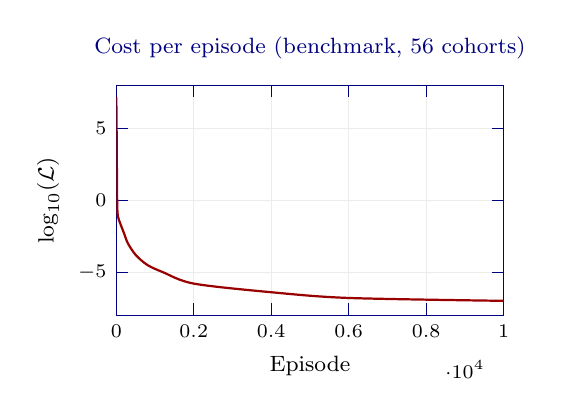
\begin{tikzpicture}
\begin{axis}[
    width=6.5cm, height=4.5cm,
    xlabel={Episode}, ylabel={$\log_{10}(\Loss)$},
    xmin=0, xmax=10000, ymin=-8, ymax=8,
    grid=major, grid style={gray!15},
    axis line style={uzhblue}, tick style={uzhblue},
    label style={font=\footnotesize}, ticklabel style={font=\scriptsize},
    title style={font=\footnotesize, uzhblue},
    title={Cost per episode (benchmark, 56 cohorts)}
]
\addplot[harvardcrimson, thick, smooth] coordinates {
    (0,7.2) (10,4.5) (20,0.5) (30,-0.8) (50,-1.2) (100,-1.6)
    (200,-2.3) (300,-3.0) (500,-3.8) (800,-4.5) (1200,-5.0)
    (2000,-5.8) (4000,-6.4) (6000,-6.8) (10000,-7.0)
};
\end{axis}
\end{tikzpicture}
\hfill
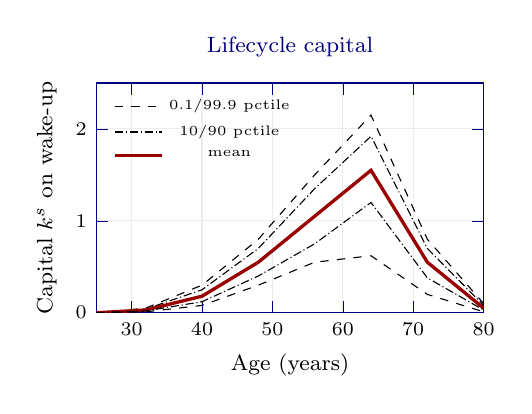
\begin{tikzpicture}
\begin{axis}[
    width=6.5cm, height=4.5cm,
    xlabel={Age (years)}, ylabel={Capital $k^s$ on wake-up},
    xmin=25, xmax=80, ymin=0, ymax=2.5,
    xtick={30,40,50,60,70,80},
    grid=major, grid style={gray!15},
    axis line style={uzhblue}, tick style={uzhblue},
    label style={font=\footnotesize}, ticklabel style={font=\scriptsize},
    title style={font=\footnotesize, uzhblue},
    title={Lifecycle capital},
    legend style={font=\tiny, draw=none, fill=none, at={(0.02,0.98)}, anchor=north west}
]
% 99.9 percentile (outer dashed)
\addplot[black, dashed, thin] coordinates {
    (25,0.00) (32,0.05) (40,0.30) (48,0.80) (56,1.50) (64,2.15) (72,0.80) (80,0.10)
};
\addlegendentry{0.1/99.9 pctile}
% 90 percentile (dash-dot)
\addplot[black, densely dashdotted, thin] coordinates {
    (25,0.00) (32,0.04) (40,0.25) (48,0.70) (56,1.35) (64,1.92) (72,0.70) (80,0.08)
};
\addlegendentry{10/90 pctile}
% mean (solid)
\addplot[harvardcrimson, very thick] coordinates {
    (25,0.00) (32,0.03) (40,0.18) (48,0.55) (56,1.05) (64,1.55) (72,0.55) (80,0.05)
};
\addlegendentry{mean}
% 10 percentile
\addplot[black, densely dashdotted, thin] coordinates {
    (25,0.00) (32,0.02) (40,0.12) (48,0.40) (56,0.75) (64,1.20) (72,0.38) (80,0.03)
};
% 0.1 percentile
\addplot[black, dashed, thin] coordinates {
    (25,0.00) (32,0.01) (40,0.08) (48,0.30) (56,0.55) (64,0.62) (72,0.20) (80,0.01)
};
\end{axis}
\end{tikzpicture}

\vspace{0.15em}
\begin{block}{Reading the plots}
\emphc{Left:} loss falls sharply but oscillates because each episode re-simulates the cloud.\\
\emphc{Right:} lifecycle capital is hump-shaped: accumulation during working years, decumulation after retirement.  Bands are simulated percentiles.
\end{block}
\end{frame}


% --- III.11 Consumption by shock state --------------------------------
\begin{frame}{III.11 Consumption Profiles by Aggregate State}
\footnotesize
\begin{block}{What the notebook will plot}
For each aggregate state $z \in \{1,2,3,4\}$ we obtain a lifecycle consumption profile $c^s(z)$ over ages $s=25,\ldots,80$, evaluated on a long ergodic simulation from notebook 08.
\end{block}

\begin{block}{The four aggregate states}
\centering\renewcommand{\arraystretch}{1.05}
\begin{tabular}{cccl}
\toprule
$z$ & $\xi(z)$ & $\delta(z)$ & expected consumption ranking \\
\midrule
2 & $1.022$ & $0.08$ & \emphc{highest} -- best technology, low depreciation \\
4 & $1.022$ & $0.11$ & high \\
1 & $0.978$ & $0.08$ & low \\
3 & $0.978$ & $0.11$ & \emphc{lowest} -- bad technology, high depreciation \\
\bottomrule
\end{tabular}
\end{block}

\begin{alertblock}{What to look for in the live plot}
Four distinct profiles, ordered as in the table above.  The exact magnitudes and crossover ages are produced by section 11 of the notebook.
\end{alertblock}
\end{frame}


% --- III.12 Reading the diagnostics -----------------------------------
\begin{frame}{III.12 Reading the Diagnostics}
\footnotesize
\begin{block}{How do we know the network actually solved the equilibrium?}
\vspace{-2pt}\begin{enumerate}\itemsep1pt
    \item \emphc{Loss level.}  $\log_{10}\Loss \lesssim -5$ means equilibrium residuals at the $10^{-3}$ level or smaller -- AGS (2022) threshold.
    \item \emphc{Per-equation Euler errors.}  Plot mean $|e_{\text{REE},k}^{\,s}|$ and $|e_{\text{REE},b}^{\,s}|$ by age $s$; expect $\sim 10^{-3}$ everywhere.
    \item \emphc{Bond market clearing.}  $|e_{\text{MC},b}| < 10^{-4}$ on the ergodic simulation path.
    \item \emphc{Borrow-binding fraction.}  Ages where $\lambda_{\text{b}}^s > 0$; standard calibration: only the youngest few cohorts.
    \item \emphc{Ergodic simulation.}  Simulate $10\,000$ periods; plot lifecycle consumption + capital with percentile bands.
\end{enumerate}
\end{block}

\vspace{-2pt}
\textbf{Hands-on: \texttt{08\_OLG\_Benchmark\_DEQN.ipynb}.}  \S 1--5 match III.1--III.5; \S 6 = cost function (III.7); \S 7--8 = training (III.9); \S 9--11 = plots and diagnostics of III.10--III.12.  Classroom runtime (128-wide, 2\,000 episodes): $\approx 30$ min on CPU.
\end{frame}


% =====================================================================
% Part IV -- Wrap-up
% =====================================================================

\section{Part IV: Wrap-up}

\begin{frame}{Summary}
\footnotesize
\begin{block}{What we accomplished}
\vspace{-2pt}\begin{enumerate}\itemsep1pt
    \item Introduced OLG as a finite-dimensional family of heterogeneous-agent models -- well suited to DEQNs because the aggregate state stays finite-dimensional.
    \item Applied the DEQN recipe \emphc{twice}:
    \begin{itemize}\itemsep0pt
        \item \emphc{Part II:} the 6-agent Krueger--K\"ubler (2004) analytic model, validated against the closed form ($\lesssim 10^{-3}$ mean Euler error).
        \item \emphc{Part III:} the 56-cohort leading-example benchmark of AGS (2022): CRRA, hump labor, persistent shocks, two assets, two borrowing constraints, capital adjustment costs.
    \end{itemize}
    \item \emphc{Same 9-step recipe} both times: setup, households I/II, firms, equilibrium, conditions, cost, FREE, architecture.
\end{enumerate}
\end{block}

\vspace{-2pt}
\begin{alertblock}{One line to remember}
\emphc{Writing down a DEQN $=$ writing down the equilibrium conditions $G$.}  Everything else (network, SGD, sampling) is boilerplate.
\end{alertblock}
\end{frame}


\begin{frame}{References and Further Reading}
\small
\begin{itemize}\itemsep3pt
    \item Azinovic, M., Gaegauf, L., \& Scheidegger, S. (2022). \emph{Deep equilibrium nets.} International Economic Review 63(4), 1471--1525.  \;[\,notebook 08 implements \S 3 of this paper].

    \item Krueger, D., \& K\"ubler, F. (2004). \emph{Computing equilibrium in OLG models with stochastic production.} Journal of Economic Dynamics \& Control 28(7), 1411--1436.  \;[\,notebook 07 implements their 6-agent analytic model].

    \item Fischer, A. (1992). \emph{A special Newton-type optimization method.} Optimization 24, 269--284.  \;[FB-complementarity function].

    \item Code: \scriptsize\url{https://github.com/sischei/DeepEquilibriumNets}.
\end{itemize}
\end{frame}


\begin{frame}{Bridge to Toolkit T1: Agentic Programming}
\footnotesize
\textbf{Where the technical content rests.}  At this point we have a complete discrete-time DEQN toolkit: feed-forward policy net + softplus output, Euler/KKT residuals + Fischer--Burmeister, simulation-based sampling, NAS-tuned architecture, and ReLoBRaLo-balanced losses, all of it scaling from a single-shock RBC sandbox up to a 56-cohort OLG benchmark with two binding constraints.

\vspace{0.4em}
\textbf{The agentic-programming toolkit (no lecture script chapter).}  We turn the workflow on its head and treat the model file, the loss, and the diagnostics as artefacts that an LLM-driven coding agent can author, refactor, and debug in conversation.  Concretely, you will:
\begin{itemize}\itemsep1pt
    \item Use Claude Code / Cursor / Codex-style agents as pair programmers on a fresh DEQN model derived from the chapters of Days 2--4.
    \item Practice the loop \emphc{specification $\to$ scaffold $\to$ run $\to$ diagnose $\to$ refactor}, with the agent doing the typing and you driving the economics.
    \item Connect the slide-deck $\to$ notebook $\to$ figure $\to$ commit pipeline that the manuscript itself was built with.
\end{itemize}

\vspace{0.4em}
\textbf{Self-study extension (notebooks 10--12, deck 08).}  Heterogeneous agents on a histogram (Young's method), continuum-of-agents DEQN, and Krusell--Smith with deep learning.  These pieces sit \emph{above} today's OLG content and can be revisited any time before the continuous-time PINN material.
\end{frame}

\end{document}
